\chapter{Passiv Radar Setup}\label{sct:setup}
Der genaue Aufbau von der Hardware bis zur Software wird in dem folgenden Kapitel erläutert werden.
\section{Hardware}
Die Hardware setzt sich zusammen aus zwei ADALM-Pluto SDR sowie zwei Yagi Antennen und einem OCXO Oscillator als externe Uhr.
\subsection{ADALM-Pluto SDR}\label{sct:sdr}
Bei dem hier verwendeten SDR handelt es sich um ein ADALM
PLUTO SDR. Der Hauptgrund, warum sich in diesem Versuchsaufbau für dieses Gerät entschieden wurde ist die Bandbreite dieses Gerätes die bei bis zu 20 MHz liegt. Die Bandbreite des Signals was hier für Passiv Radar verwendet wird beträgt  5 MHz was einige SDR nicht aufbringen können.  Aufs weitere besitzt das SDR eine Frequenz Abdeckung von 325 KHz bis zu 3.8 MHz. Die weiteren Daten können in der Tabelle abgelesen werden. 
\subsubsection{Synchronität}\label{sct:Oscillator}
Zur Aufnahme des Referenzsignals als auch des reflektierten Signals werden jeweils ein Pluto-SDR benötigt, diese zwei müssen nun synchron betrieben werden. Dies wird erreicht durch Daisy Chaining  der beiden Uhren der SDRs und einem OCXO Oscillator als externen Uhr. Die Abbildungen ~\ref{fig:Pluto} zeigen dann den fertigen Aufbau der Beiden SDRs und im Schaltplan in Abbildung ~\ref{fig:Clock} ist zur erkennen wie die Uhr der jeweiligen SDRs aufgebaut ist.

\begin{figure}
    \centering
    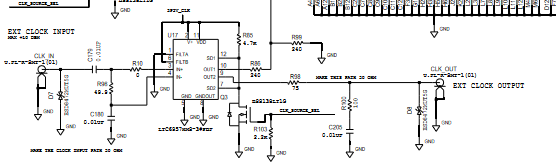
\includegraphics[width=\textwidth]{images/Schaltplan_Clock.png}
    \caption{Schaltplan der Clock des Pluto SDRs} \label{fig:Clock}
\end{figure}

\begin{figure}
    \centering
    \begin{subfigure}[Pluto mit Clock]{0.3\textwidth}
        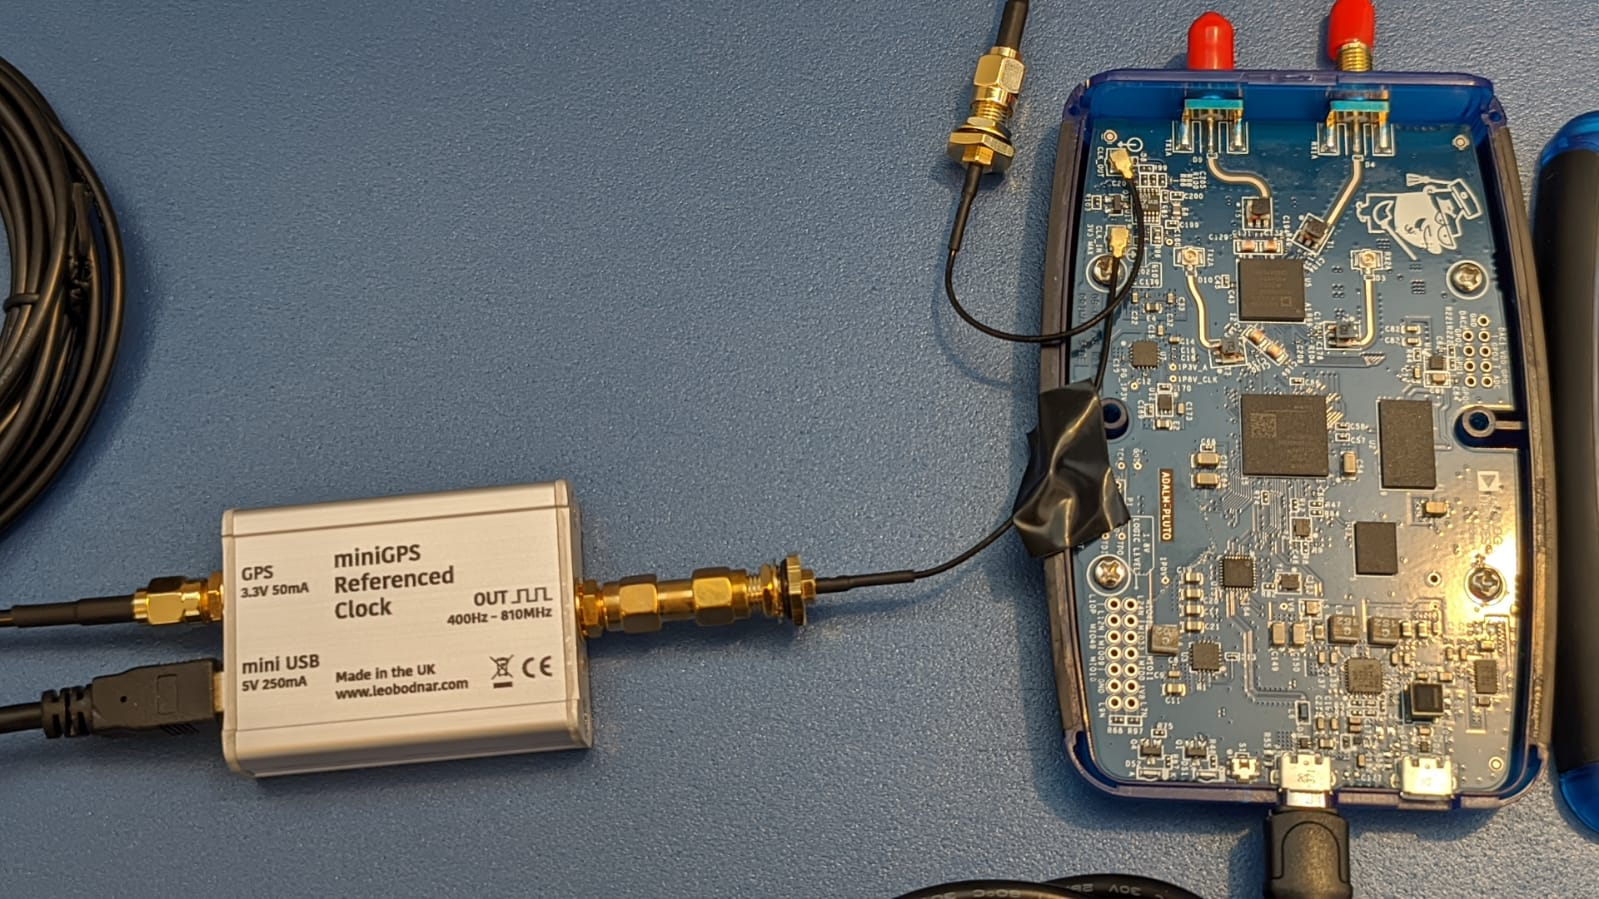
\includegraphics[width=\textwidth]{images/Pluto_1.jpeg}
        \caption{Pluto SDR und OCXO Oscillator}
    \end{subfigure}
    \begin{subfigure}[Daisy Chaining]{0.3\textwidth}
        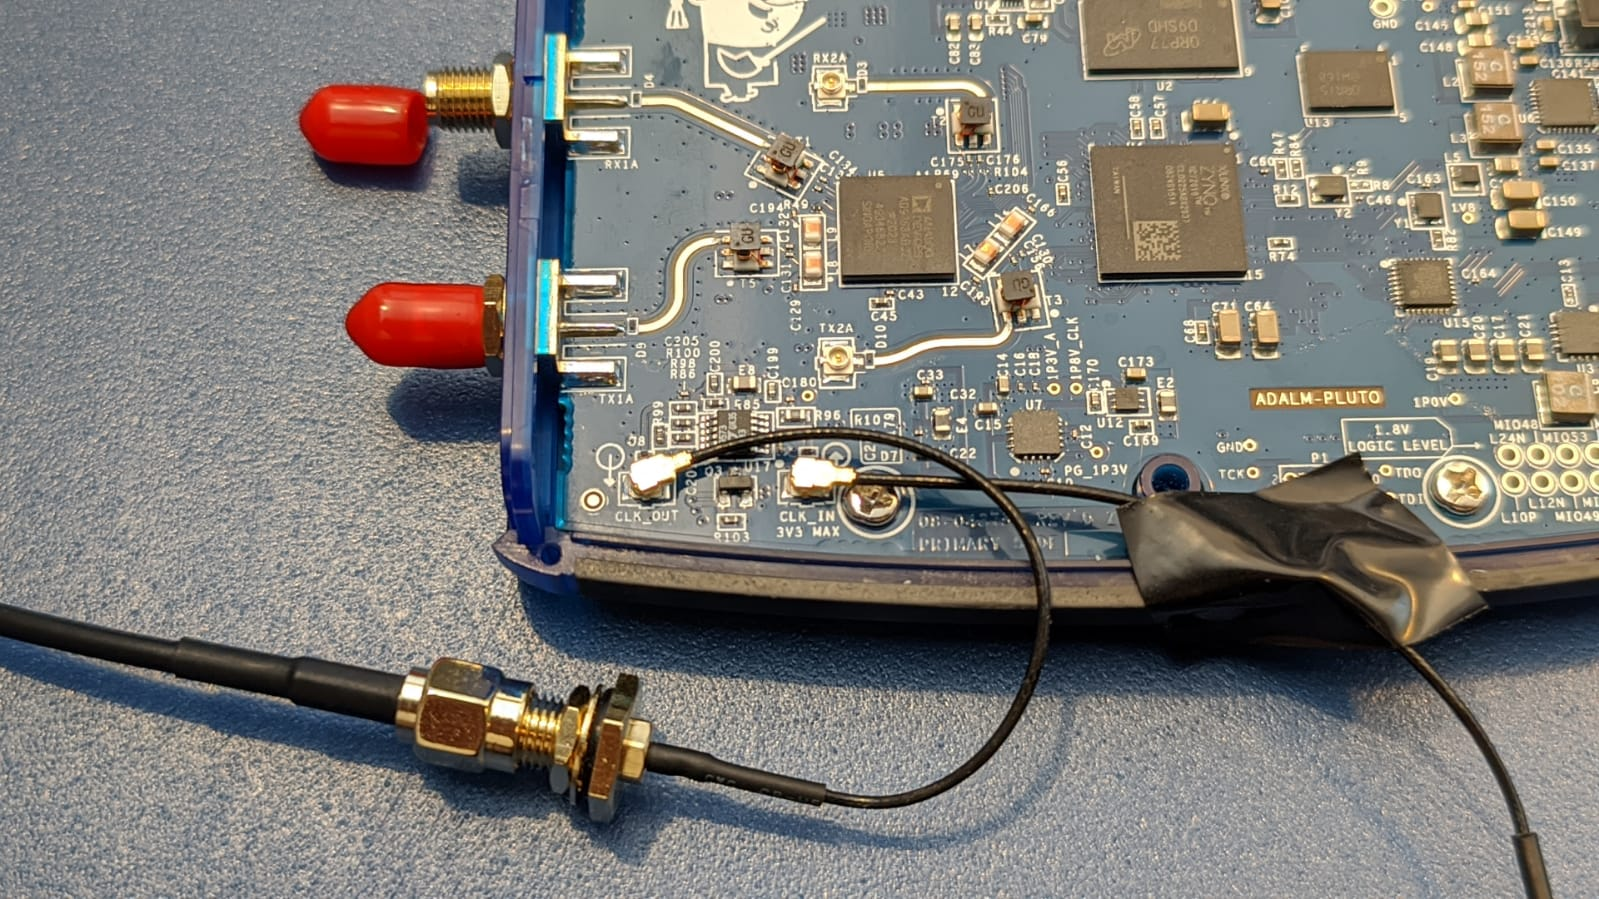
\includegraphics[width=\textwidth]{images/Pluto_2.jpeg}
        \caption{Daisy Chaining}
    \end{subfigure}
    \begin{subfigure}[Gesamter Aufbau]{0.3\textwidth}
        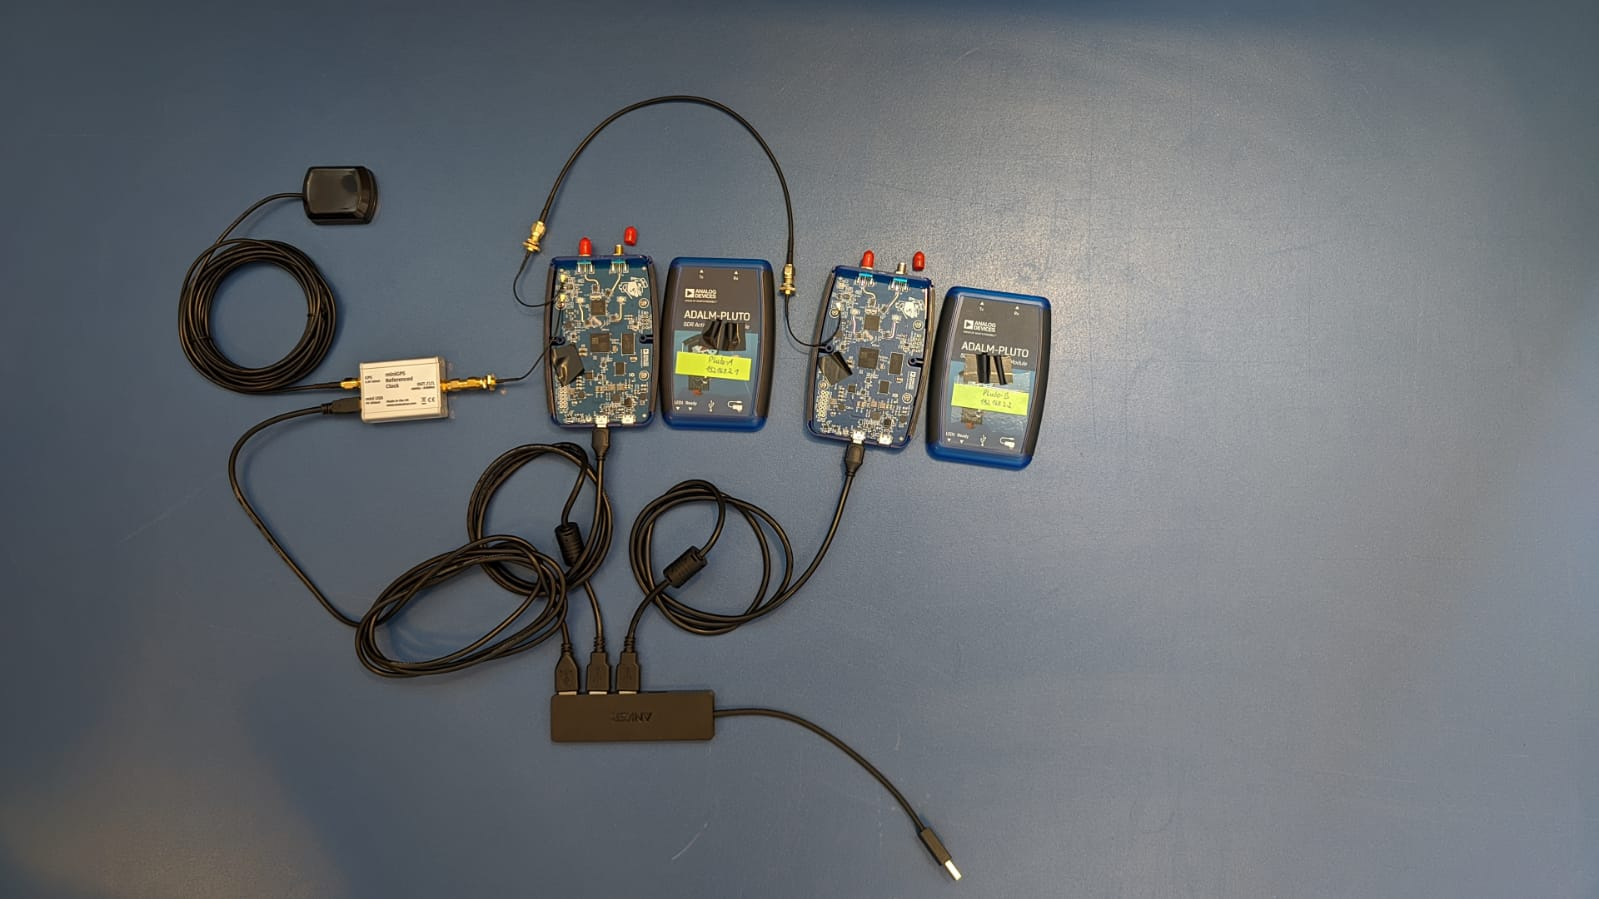
\includegraphics[width=\textwidth]{images/Pluto_4.jpeg}
        \caption{Der gesamte Aufbau}
    \end{subfigure}
    \caption{Aufbau der Hardware mit den beiden Plutos und der Clock} \label{fig:Pluto}
\end{figure}

\subsection{Antenne}
In diesem Aufbau werden zwei Antennen die für DVB-T gedacht sind verwendet. Die Antenne ist ein Yagi Antenne mit 43 Elementen wie man im Abbildung ~\ref{fig:antenne} sieht die im Frequenzbereich von 470 bis 862 MHZ arbeitet, was für unseren Anwendungsfall sehr gut geeignet ist. Die weiteren Daten zur Antenne stehen in der Tabelle ~\ref{table:antenne}.

\begin{table}
    \centering
        \begin{tabular}[h]{rl}
            Antenne         & SKT SL43-01 UHF 43            \\
            Antennengewinn  & 11..13 dB                     \\
            Frequenzbereich & 470-862 MHz                   \\
            Halbwertsbreite & horiz. 30...40°/ver. 35...50° \\
        \end{tabular}
    \caption{Daten der SKT SL43-01 UHF 43 Antenne}\label{table:antenne}
\end{table}

\begin{figure}
    \centering
    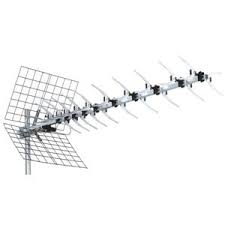
\includegraphics[width=\textwidth]{images/antenne.png}
    \caption{SKT SL43-01 UHF 43 Antenne}\label{fig:antenne}
\end{figure}
\section{Signal}
Das hier verwendete Signal beruht auf der LTE Technik. LTE besteht aus OFDM Modulen und benutzt die MIMO Technik. Ein LTE Frame ist 1ms lang und besteht aus 10 subframes.
\subsection{Aufbau von LTE}
Ein LTE-Signal besteht aus 504 unterschiedlichen Zellidentitäten auf physikalischer Ebene, diese sind in 168 unterschiedliche physikalischer Gruppen unterteilt. Eine Zellidentität setzt sich zusammen aus Identifikationsnummer der Gruppe sowie der Identifikationsnummer der jeweiligen physikalischen Ebene in der physikalischen Gruppe zusammen. Somit berechnet sich die Zellidentität wie folgt: $$N_{ID}^{cell}=3N_{ID}^{(1)}+N_{ID}^{(2)}$$ Hierbei gilt, dass jede Gruppe eine Nummer $N_{ID}^{(1)}$ zur Identifikation im Bereich von 0 bis 167 besitzt. Außerdem liegt die Identifikationsnummer $N_{ID}^{(2)}$ der physikalischen Ebene in der physikalischen Gruppe im Bereich von 0 bis 2.
Zur Synchronisation des Signals benutzt LTE sowohl ein Primary Synchronisation Signal (PSS) als auch ein Secondary Synchronisation Signal (SSS).~\cite[S.~180]{etsi2021136}
\subsection{OFDM}
\begin{figure}
    \centering
    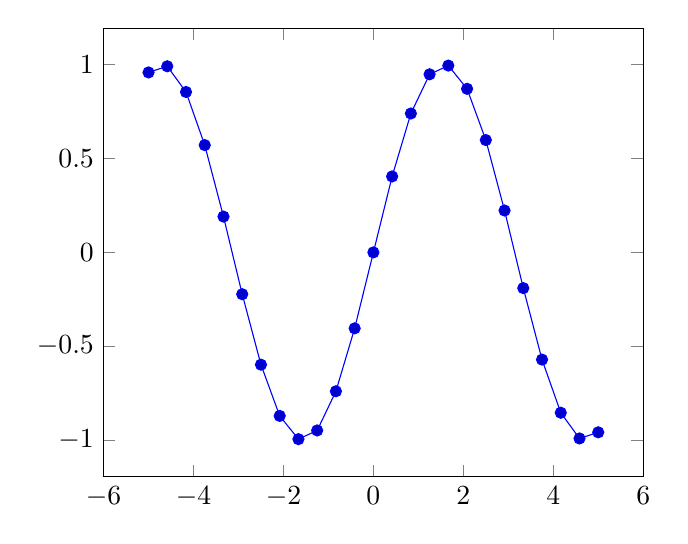
\begin{tikzpicture}
        \begin{axis}
            \addplot {sin(deg(x))};
        \end{axis}
    \end{tikzpicture}
\end{figure}

\subsubsection{Primary Synchronisation Signal (PSS)}
 PSS wird in jeden Frame zweimal übertragen, und zwar im ersten und 10 Slot. Innerhalb jedes Slots wird das PSS im letzten OFDM Symbol übertragen. Was UE damit erreicht mit dem PSS erreicht ist eine Subframe Synchronisation, eine Slot Synchronisation sowie eine Symbol Synchronisation. Außerdem kann die Mitte des jeweiligen Kanals bestimmt werden in der Frequenz Domain. Ebenfalls wird die passenden PCI aus den drei verschiedenen PCI erkannt.
 Die Sequenz des PSS wird generiert durch die Zadoff-Chu erzeugt. Zadoff-Chu: $$ 	\operatorname{d_u}(n)=\begin{cases} e^{-j}, & \mbox{wenn }n\mbox{ gerade} \\ e^{-j}, & \mbox{wenn }n\mbox{ ungerade} \end{cases}$$
\subsubsection{Secondary Synchronisation Signal (SSS)}


\section{Software}
\subsection{SDR-angel}
Die Aufnahmen in diesem Projekt wurden mit der Open-Source-Software SDR-Angel gemacht. Mit der auch beide SDRs parrallel aufgezeichnen werden können.
\subsection{Signalverarbeitung}
\subsubsection{Ambiguity Funktion}\label{sct:ambiguity_function}
\subsubsection{Clean Algorithmus}
